% CAPITULO IMPLEMENTACION 

\chapter{Detalles de implementaci�n}\label{chap:detallesImpl}

\begin{flushright}
  \begin{minipage}[t]{13cm}
    \begin{flushright}
      \begin{quote}
        \emph{
          Se deben absorber los colores de la vida, pero nunca deben de
          recordarse sus detalles. Los detalles son siempre vulgares.
        }
        \begin{flushright}
          \textbf{\textemdash Oscar Wilde, El retrato de Dorian Gray}
        \end{flushright}
      \end{quote}
    \end{flushright}
  \end{minipage}
\end{flushright}

\bigskip

\begin{flushright}
  \begin{minipage}[t]{13cm}
    \begin{flushright}
      \begin{quote}
        \emph{
          Cu�date de aquel que no se molesta en los detalles.
        }
        \begin{flushright}
          \textbf{\textemdash William Feather}
        \end{flushright}
      \end{quote}
    \end{flushright}
  \end{minipage}
\end{flushright}

\bigskip

\begin{center}{\line(1,0){325}}\end{center}

%--------------------------------------------------------%
\section{Introducci�n}
 

\section{Elementos generados din�micamente}
 
  - system info
    - cpu info
    - compilation config
  - preprocesador en python => necesario por uso de aop
  - el cliente en python
  - el mecanismo de perfilado basado en aop


\section{Asegurando la coherencia algebraica}
- comprobaciones estataticas de caracter algebraico de parametros de templates
en la particularizaci�n de estructuras genericas


\section{El nuevo repositorio de funciones}\ref{nuevoRepdeFuncs}

\section{La CPU SIMD}
Descrita en la secci�n \ref{basico:cpusimd}, esta CPU virtual consigue trabajar
no s�lo con sus operandos de forma intr�nsecamente paralela sino tambi�n con
tres tipos diferentes de datos. Todo ello con una interfaz com�n que aisla 
al usuario programador de los entresijos de su funcionamiento. Sin embargo no se
consigue este comportamiento por arte de m�gia.

\subsection{El tipo \texttt{SIMDDigit}}
\subsection{El problema del alineamiento}
\subsection{Mismo fin, diferentes medios}
no solo el soporte de tres tipos, sino tambien la forma subyacente de procesarlos
en funci�n de las tecnologias disponibles.





\section{La utilidad de fingir}
- mock openmp


\section{El mundo de los $64$ bits}

\section{El maestro compilador}
- scons

\section{Implementaci�n de tipos}
  \subsection{El tipo \emph{\texttt{MPPDataType}}\index{tipos!MPPDataType} }

  \subsection{Categorizaci�n algebraica}\label{categorizacionAlgebraica}
  En la figura \ref{fig:categoriasAlgebraicas} se muestra la jerarqu�a de clases que
  modelan las categor�as algebraicas consideradas, junto con sus m�todos (est�ticos) asociados.  
  \begin{figure}[h]
    \centering
    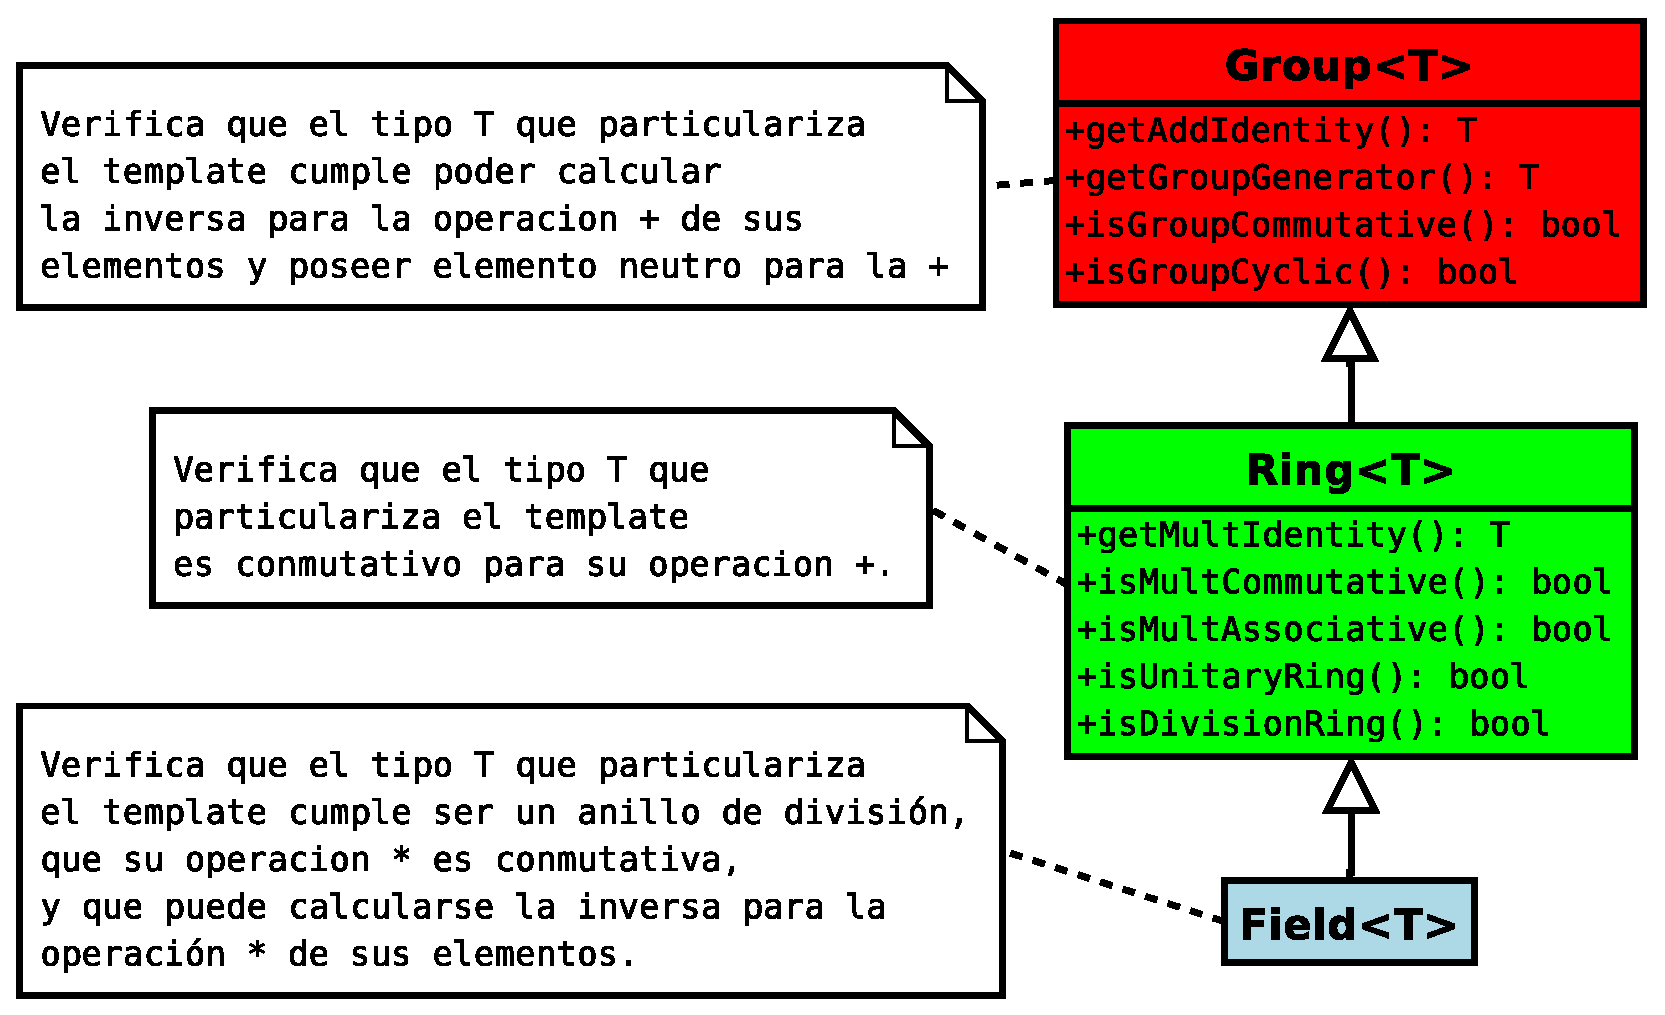
\includegraphics[width=0.95\textwidth,keepaspectratio]{categoriasAlgebraicas} 
    \caption{Categorias algebraicas}\label{fig:categoriasAlgebraicas}
  \end{figure}
  Cuando un tipo de dato de la librar�a (es decir, un hijo de \texttt{MPPDataType}) se
  encasilla dentro de esta jerarqu�a, sobre dicho tipo (representado mediante el par�metro 
  de plantilla \texttt{T}) se realizan una serie de comprobaciones, dise�adas para verificar
  que efectivamente dicho tipo cumple las condiciones impuestas por la categor�a 
  algebraica a la que aspira pertenecer. Esta serie de comprobaciones se realizan por medio
  de \emph{asertos}.



\begin{lstlisting}[captionpos=b,basicstyle=\footnotesize,frame=shadowbox,rulesepcolor=\color{black},language=C++,numbers=left,caption=STATIC\_ASSERT, label=lst:staticassert]
~Group() {
  STATIC_ASSERT( ValidateRequirements() );
}
(...)
static bool ValidateRequirements() {
  T (T::*getAddInverse)() const = &(T::getAddInverse) ;
  const T& (*getAddIdentity)() = &(T::getAddIdentity) ;
  const T& (*getGroupGenerator)() = &(T::getGroupGenerator) ;

  return true;
}
\end{lstlisting}


  \begin{figure}[h]
    \centering
    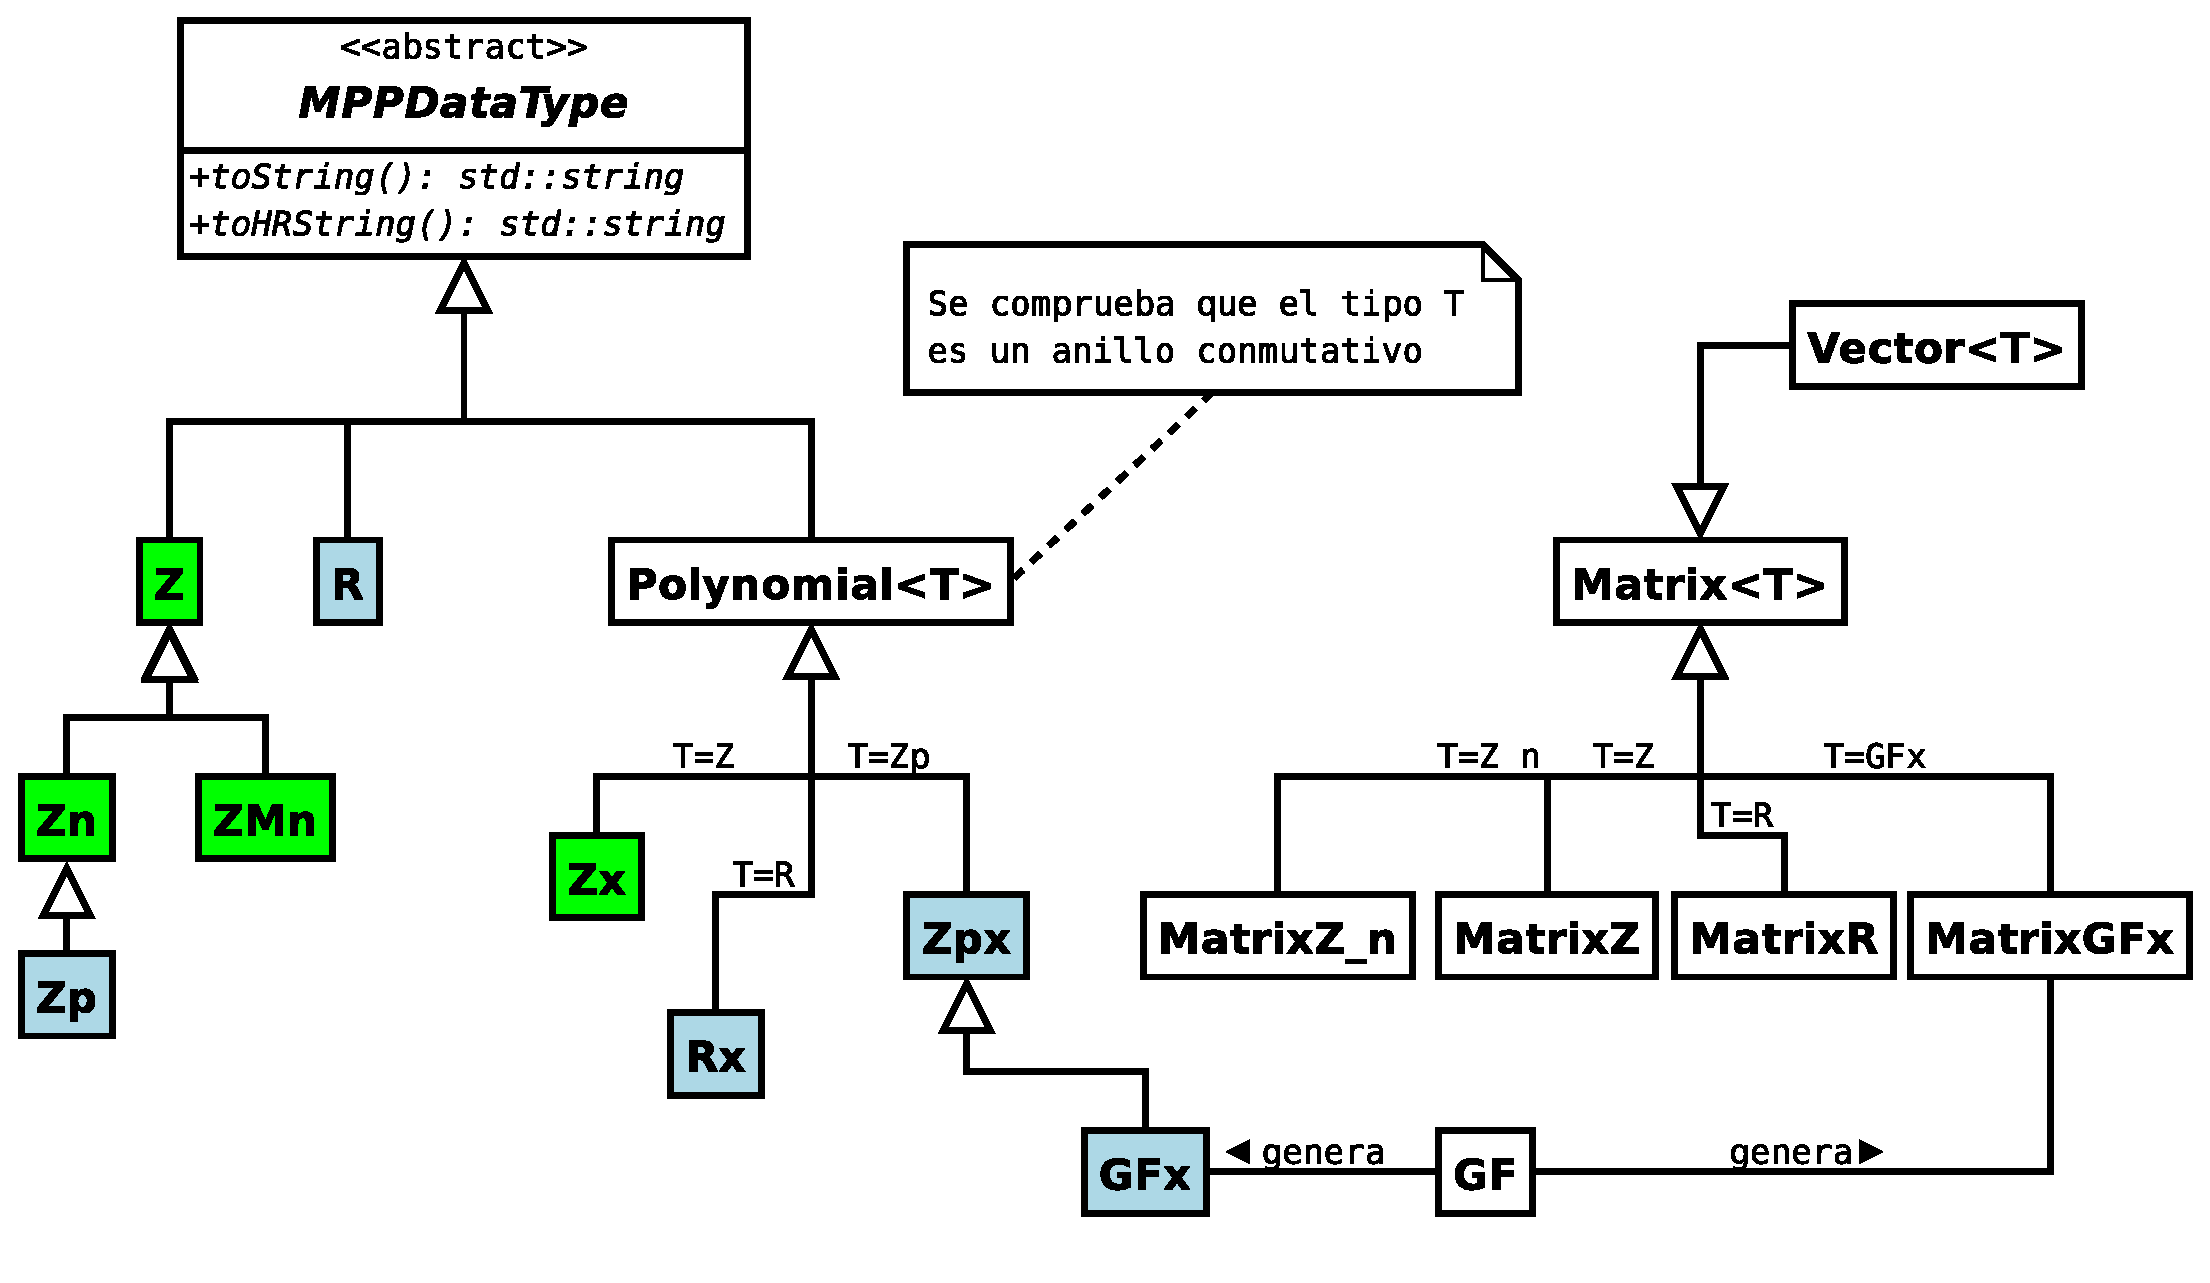
\includegraphics[width=0.95\textwidth,keepaspectratio]{categorizacionAlgebraica} 
    \caption{Categorizaci�n algebraica}\label{fig:categorizacionAlgebraica}
  \end{figure}




  \subsection{Enteros $\mathbb{Z}M_n$}\label{implZM_n}

  \subsection{Polinomios}\index{implementaci�n!polinomios}\label{impl:polinomios}
    totalmente genericos
  \subsubsection{Verificando el car�cter de $S$}
    tiene que ser como ser como minimo anillo conmutativo con unidad. Verificaciones estaticas

 El requerir que $S$ sea un tipo de la biblioteca responde simplemente a que en la posterior
  implementaci�n de los m�todos, se depende de las caracter�sticas comunes de los tipos de la biblioteca.



  \subsubsection{Operaciones dependientes de $S$}
    p ej, div en udf o  no, idem pa gcd  


  \subsection{Matrices}\index{tipos!Matrices}
